\documentclass[aspectratio=169,11pt]{beamer}

\usetheme[progressbar=frametitle,numbering=fraction,block=fill]{metropolis}
\usepackage[T1]{fontenc}
\usepackage[sfdefault,lining]{FiraSans}
\usepackage[scale=0.85]{FiraMono}
\usepackage{newtxsf}
\usepackage{booktabs,multirow,tabularx,array}
\usepackage{siunitx}
\usepackage{pifont}
\usepackage{tikz}
\usetikzlibrary{positioning,calc}
\usepackage[dvipsnames]{xcolor}

\graphicspath{{../report/figures/}}
% Generated by scripts/make_figures.py -- do not edit by hand.
\newcommand{\alignSlope}{1.8}
\newcommand{\alignTimeMax}{0.5}
\newcommand{\arGEnd}{473}
\newcommand{\arGLen}{23}
\newcommand{\arGStart}{451}
\newcommand{\arQEnd}{80}
\newcommand{\arQLen}{23}
\newcommand{\arQStart}{58}
\newcommand{\arRawEnd}{473}
\newcommand{\arRawIdentity}{31}
\newcommand{\arRawLen}{430}
\newcommand{\arRawOffset}{1}
\newcommand{\arRawStart}{44}
\newcommand{\arRawZ}{66}
\newcommand{\colAlnIdentity}{55}
\newcommand{\colAlnScore}{87}
\newcommand{\colAlnZ}{7.4}
\newcommand{\colGlyFraction}{100.0}
\newcommand{\colPeakPeriod}{3.00}
\newcommand{\colPeakPower}{102}
\newcommand{\colRegionEnd}{1183}
\newcommand{\colRegionLen}{997}
\newcommand{\colRegionScore}{0.33}
\newcommand{\colRegionStart}{187}
\newcommand{\colSecondPower}{19}
\newcommand{\entropyTimeMax}{2}
\newcommand{\httAlnZ}{1.1}
\newcommand{\httLcrEnd}{85}
\newcommand{\httLcrStart}{11}
\newcommand{\httPEnd}{49}
\newcommand{\httPLen}{11}
\newcommand{\httPStart}{39}
\newcommand{\httQEnd}{38}
\newcommand{\httQLen}{21}
\newcommand{\httQStart}{18}
\newcommand{\nShuffles}{50}
\newcommand{\runtimeMaxLength}{4{,}000}
\newcommand{\supAlnA}{3--82}
\newcommand{\supAlnB}{21--101}
\newcommand{\supAlnIdentity}{52}
\newcommand{\supAlnOffset}{18}
\newcommand{\supAlnScore}{180}
\newcommand{\supAlnZ}{6.5}
\newcommand{\supUnit}{QQYNPQGGY}
\newcommand{\supUnitEnd}{90}
\newcommand{\supUnitStart}{71}
\newcommand{\tandemMinLength}{8}
\newcommand{\toyLength}{66}
\newcommand{\toyNyquistIndicator}{1.9}
\newcommand{\toyNyquistKD}{0.1}
\newcommand{\zSignificant}{4}


% ---------------------------------------------------------------- colours
\definecolor{accent}{HTML}{2A78D6}
\definecolor{accent2}{HTML}{EB6834}
\definecolor{accent3}{HTML}{1BAF7A}
\definecolor{inkmuted}{HTML}{52514E}
\definecolor{accent4}{HTML}{C98500}
\definecolor{ink}{HTML}{1B1B1A}
\definecolor{paper}{HTML}{FCFCFB}
\setbeamercolor{normal text}{fg=ink, bg=paper}
\setbeamercolor{alerted text}{fg=accent2}
\setbeamercolor{example text}{fg=accent}
\setbeamercolor{frametitle}{bg=ink, fg=paper}
\setbeamercolor{progress bar}{fg=accent, bg=accent!20}
\setbeamercolor{title separator}{fg=accent}
\setbeamercolor{block title}{bg=accent!12, fg=ink}
\setbeamercolor{block body}{bg=accent!5}
\setbeamerfont{caption}{size=\scriptsize}
\setbeamertemplate{caption}{\insertcaption}

\newcommand{\cmark}{\textcolor{accent3}{\ding{51}}}
\newcommand{\xmark}{\textcolor{inkmuted}{\ding{55}}}
\newcommand{\seq}[1]{\texttt{#1}}
\newcommand{\muted}[1]{\textcolor{inkmuted}{#1}}

\title{Amino Acid Repeats}
\subtitle{Analysis \& Implications}
\author{Ali Ahmadi Esfidi}
\date{Feb, 2025}

\begin{document}

\maketitle

% ---------------------------------------------------------------- 1
\begin{frame}{Abstract}
\vfill
Amino acid repeats (AARs) are abundant in protein sequences and play key roles in protein
function and evolution.

\medskip
This work reviews and implements \alert{four detection methodologies}, evaluates them on a synthetic
benchmark and four real proteins, and discusses the biological implications, including disease associations
through repeat variation.
\vfill
\begin{columns}[T]
\column{0.24\textwidth}\centering\textbf{\color{accent2}Entropy}\\\muted{\small low complexity}
\column{0.24\textwidth}\centering\textbf{\color{accent}Self-match}\\\muted{\small tandem units}
\column{0.24\textwidth}\centering\textbf{\color{accent3}Fourier}\\\muted{\small periodicity}
\column{0.24\textwidth}\centering\textbf{\color{accent4}Self-alignment}\\\muted{\small diverged copies}
\end{columns}
\vfill
\end{frame}

% ---------------------------------------------------------------- 2
\begin{frame}{Introduction}
\begin{columns}[T]
\column{0.52\textwidth}
\textbf{AAR prevalence \& significance}
\begin{itemize}
  \item Common in structural and functional proteins, more so in eukaryotes
  \item Range from \alert{simple runs} (\seq{QQQQQ}) to \alert{complex domain repeats} (20--40\,aa units)
  \item Variation links to \alert{function and disease}: copy number changes far faster than point mutation
\end{itemize}
\column{0.44\textwidth}
\begin{block}{Example: huntingtin (HTT)}
\small
\seq{MATLEKLMKAFESLKSF}\\
\seq{\textcolor{accent2}{QQQQQQQQQQQQQQQQQQQQQ}}\\
\seq{\textcolor{accent}{PPPPPPPPPPP}QLPQPPPQAQP\dots}

\medskip
A \seq{Q$_{\httQLen}$} tract (residues \httQStart--\httQEnd) whose expansion beyond about 36 causes Huntington's disease.
\end{block}
\end{columns}
\end{frame}

% ---------------------------------------------------------------- 3
\begin{frame}{Classification framework}
\centering
\resizebox{0.86\linewidth}{!}{% Classes of amino acid repeats (shared by report and slides).
% Requires colours accent, accent2, accent3, inkmuted and xcolor's dvipsnames.
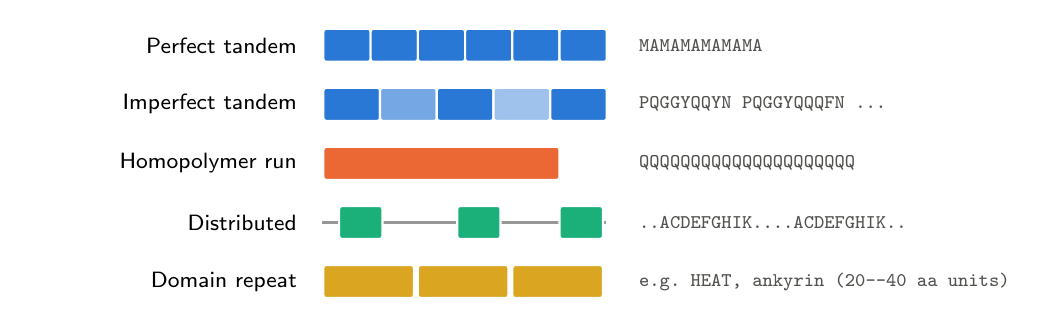
\begin{tikzpicture}[
  font=\sffamily\small,
  unit/.style={draw=white, line width=0.8pt, minimum height=0.42cm, inner sep=0pt, rounded corners=1pt},
  lab/.style={anchor=east, text width=3.3cm, align=right, font=\sffamily\footnotesize},
  note/.style={anchor=west, font=\ttfamily\scriptsize, text=inkmuted}]
  \def\row#1{-0.75*#1}
  % perfect tandem
  \node[lab] at (-0.2,{\row0}) {Perfect tandem};
  \foreach \i in {0,...,5} \node[unit, fill=accent, minimum width=0.6cm, anchor=west] at (0.6*\i,{\row0}) {};
  \node[note] at (3.9,{\row0}) {MAMAMAMAMAMA};
  % imperfect tandem
  \node[lab] at (-0.2,{\row1}) {Imperfect tandem};
  \foreach \i/\c in {0/accent,1/accent!65,2/accent,3/accent!45,4/accent} \node[unit, fill=\c, minimum width=0.72cm, anchor=west] at (0.72*\i,{\row1}) {};
  \node[note] at (3.9,{\row1}) {PQGGYQQYN PQGGYQQQFN \dots};
  % homopolymer
  \node[lab] at (-0.2,{\row2}) {Homopolymer run};
  \node[unit, fill=accent2, minimum width=3.0cm, anchor=west] at (0,{\row2}) {};
  \node[note] at (3.9,{\row2}) {QQQQQQQQQQQQQQQQQQQQQ};
  % dispersed
  \node[lab] at (-0.2,{\row3}) {Distributed};
  \draw[inkmuted!60, line width=1.2pt] (0,{\row3}) -- (3.6,{\row3});
  \foreach \x in {0.2,1.7,3.0} \node[unit, fill=accent3, minimum width=0.55cm, anchor=west] at (\x,{\row3}) {};
  \node[note] at (3.9,{\row3}) {..ACDEFGHIK....ACDEFGHIK..};
  % domain
  \node[lab] at (-0.2,{\row4}) {Domain repeat};
  \foreach \i in {0,1,2} \node[unit, fill=Goldenrod, minimum width=1.15cm, anchor=west] at (1.2*\i,{\row4}) {};
  \node[note] at (3.9,{\row4}) {e.g.\ HEAT, ankyrin (20--40 aa units)};
\end{tikzpicture}
}

\vfill
\begin{columns}[T]
\column{0.31\textwidth}\centering\textbf{Unit similarity}\\\muted{\small perfect vs.\ imperfect}
\column{0.31\textwidth}\centering\textbf{Spatial arrangement}\\\muted{\small tandem vs.\ distributed}
\column{0.31\textwidth}\centering\textbf{Pattern complexity}\\\muted{\small simple vs.\ domain repeats}
\end{columns}
\vfill
\muted{\footnotesize Each detection strategy is sensitive to a different combination of these axes.}
\end{frame}

% ---------------------------------------------------------------- 4
\begin{frame}{Detection strategies}
\centering\small
\renewcommand{\arraystretch}{1.2}
\begin{tabularx}{\textwidth}{@{}l>{\raggedright\arraybackslash}X>{\raggedright\arraybackslash}X@{}}
\toprule
\textbf{Methodology} & \textbf{Idea} & \textbf{Finds} \\
\midrule
\textcolor{accent2}{\textbf{Complexity measurement}} & Sliding-window Shannon entropy (SEG thresholds) & Homopolymers, low-complexity regions \\
\textcolor{accent}{\textbf{Shifted self-match}} & Compare $s_i$ with $s_{i+p}$ for every period $p$ & Exact tandem units, copy number \\
\textcolor{accent3}{\textbf{Fourier transform}} & Spectral energy at harmonics of $1/p$ & Periodic patterns without identical units \\
\textcolor{accent4}{\textbf{Self-comparison alignment}} & Smith--Waterman of $s$ against itself & Diverged tandem \& distributed copies \\
\muted{\textbf{Machine learning}} & \muted{Profiles, structure prediction, classifiers} & \muted{Very diverged domain repeats (outlook)} \\
\bottomrule
\end{tabularx}
\end{frame}

% ---------------------------------------------------------------- 5
\begin{frame}{Complexity measurement: Shannon entropy}
\begin{columns}[c]
\column{0.33\textwidth}
\[ H(w) = -\sum_{a} f_a \log_2 f_a \]
\small
\begin{itemize}
  \item $H=0$ for a homopolymer, $H=1$ for \seq{ABAB\dots}
  \item \alert{Trigger} $H\le 2.2$ seeds a region; \alert{extension} $H\le 2.5$ grows it ($W=12$)
  \item Linear time
\end{itemize}
\column{0.65\textwidth}
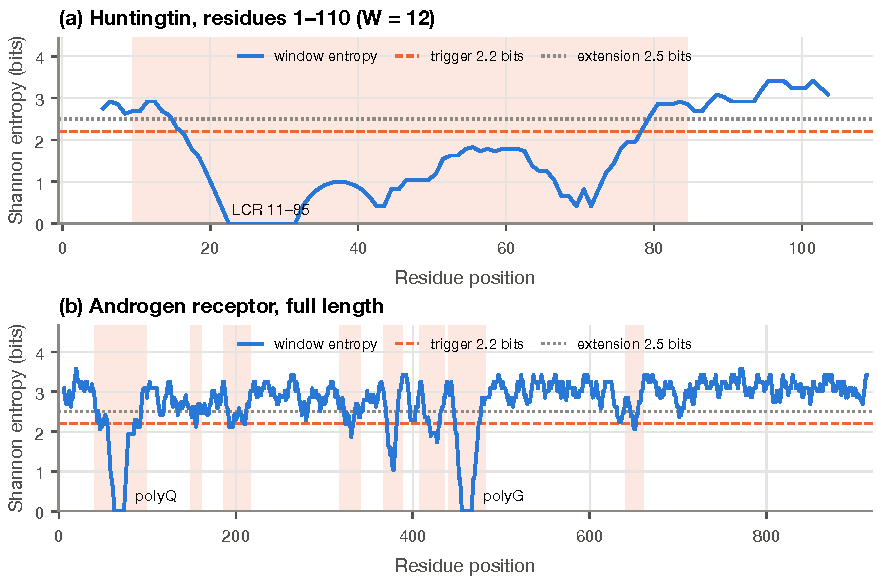
\includegraphics[width=\linewidth]{entropy.pdf}
\end{columns}
\end{frame}

% ---------------------------------------------------------------- 6
\begin{frame}{Fourier transform pattern recognition}
\begin{columns}[c]
\column{0.47\textwidth}
\small
\textbf{Encoding:} one indicator channel per residue, $x_{a,j} = [s_j = a]$\\
\muted{\footnotesize (hydropathy barely separates \seq{M/A}, \seq{S/T})}

\smallskip
\textbf{Local periodicity score}
\[ S_p = \frac{\sum_a \sum_{k=1}^{p-1} |X_a(k/p)|^2}{W_p \sum_{a,j} (x_{a,j}-\bar x_a)^2} \in [0,1] \]
By Parseval: the \alert{fraction of variance explained by period $p$};
$S_p=1$ for a perfect repeat, $\approx (p-1)/W_p$ at random.

\smallskip
Spectrum \emph{proposes} periods, string matching \emph{verifies} them.
\column{0.5\textwidth}
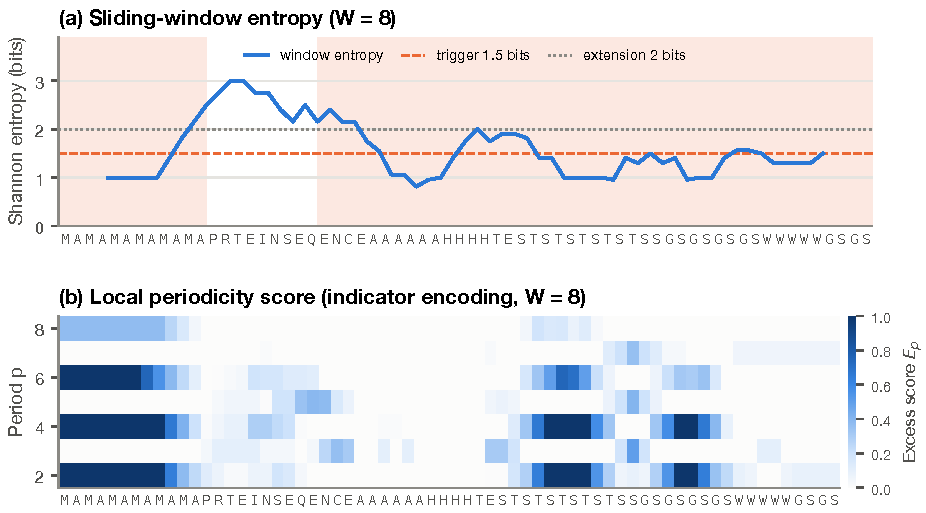
\includegraphics[width=\linewidth]{toy.pdf}
\end{columns}
\end{frame}

% ---------------------------------------------------------------- 7
\begin{frame}{Fourier: the collagen triple helix}
\centering
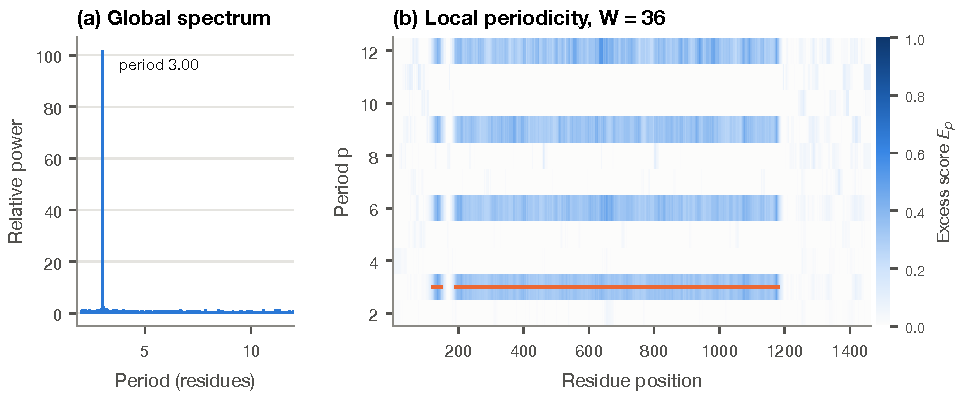
\includegraphics[height=0.56\textheight]{fourier_collagen.pdf}

\medskip
\begin{columns}[T]
\column{0.32\textwidth}\centering
\textbf{\Large\color{accent}\colPeakPower$\times$}\\\muted{\small power at period \colPeakPeriod}
\column{0.32\textwidth}\centering
\textbf{\Large\color{accent}\colRegionStart--\colRegionEnd}\\\muted{\small period-3 region}
\column{0.32\textwidth}\centering
\textbf{\Large\color{accent}\colGlyFraction\,\%}\\\muted{\small Gly in one triplet phase}
\end{columns}

\smallskip
\muted{\footnotesize Gly-X-Y has no identical units: only the spectrum reveals the architecture.}
\end{frame}

% ---------------------------------------------------------------- 8
\begin{frame}{Self-comparison alignment}
\begin{columns}[c]
\column{0.36\textwidth}
\small
\begin{itemize}
  \item Smith--Waterman, BLOSUM62, upper triangle only
  \item \alert{Waterman--Eggert declumping}: no shadow alignments
  \item Significance: $z$-score vs.\ \nShuffles{} shuffles
\end{itemize}
\begin{block}{Sup35 oligopeptide repeats}
\footnotesize
\supAlnA{} $\sim$ \supAlnB{},
offset \supAlnOffset{} (two units), identity \supAlnIdentity\,\%, $z = \supAlnZ$
\end{block}
\column{0.62\textwidth}
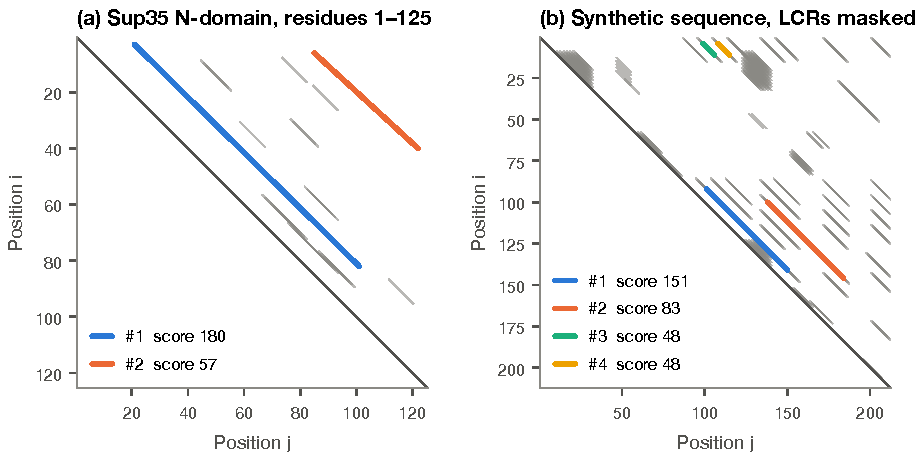
\includegraphics[width=\linewidth,height=0.8\textheight,keepaspectratio]{dotplot.pdf}
\end{columns}
\end{frame}

% ---------------------------------------------------------------- 9
\begin{frame}{Pitfall: low-complexity regions dominate alignments}
\begin{columns}[c]
\column{0.48\textwidth}
\begin{block}{Androgen receptor, unmasked}
Best self-alignment spans residues \arRawStart--\arRawEnd{} (\arRawLen{} aa) at offset \arRawOffset, identity \arRawIdentity\,\%.

\smallskip
PolyQ, polyP and polyG tracts are \alert{chained into one ``repeat''} with apparent $z = \arRawZ$.
\end{block}
\column{0.48\textwidth}
\begin{block}{After SEG masking}
\begin{itemize}\small
  \item AR: no alignment above threshold
  \item Collagen: Gly-X-Y homology, $z = \colAlnZ$
  \item HTT HEAT-like repeats: $z = \httAlnZ$ (too diverged for pairwise alignment)
\end{itemize}
\end{block}
\end{columns}
\vfill
\centering\muted{Mask LCRs before alignment, as BLAST and RADAR do.}
\end{frame}

% ---------------------------------------------------------------- 10
\begin{frame}{Synthetic benchmark: who finds what?}
\centering
\small
\resizebox{\textwidth}{!}{\begin{tabular}{@{}lllccccc@{}}
\toprule
Element & Residues & Class & Entropy & Tandem & Fourier & Self-align. & Words \\
\midrule
(MA)$_6$ & 1--12 & perfect tandem & \cmark & \cmark & \cmark & \cmark & \cmark \\
(A)$_6$ & 26--31 & homopolymer & \cmark & \cmark & \xmark & \cmark & \cmark \\
(H)$_4$ & 32--35 & homopolymer & \cmark & \cmark & \xmark & \cmark & \xmark \\
(ST)$_{5}$S & 38--48 & perfect tandem & \cmark & \cmark & \cmark & \cmark & \cmark \\
(SG)$_{4}$S & 49--57 & perfect tandem & \cmark & \cmark & \cmark & \cmark & \cmark \\
(W)$_5$ & 58--62 & homopolymer & \cmark & \cmark & \xmark & \cmark & \xmark \\
PRTEINSEQENCE & 13--25 & non-repeat spacer & \xmark & \xmark & \xmark & \cmark & \xmark \\
\bottomrule
\end{tabular}
}

\medskip
\muted{\scriptsize\seq{MAMAMAMAMAMAPRTEINSEQENCEAAAAAAHHHHTESTSTSTSTSTSSGSGSGSGSWWWWWGSGS}}\\[0.3em]
\muted{\footnotesize The spacer is a negative control: the self-alignment \cmark{} there is a false positive.}
\end{frame}

% ---------------------------------------------------------------- 11
\begin{frame}[t]{Results on real proteins}\vspace{-0.6em}
\begin{columns}[c]
\column{0.62\textwidth}
\centering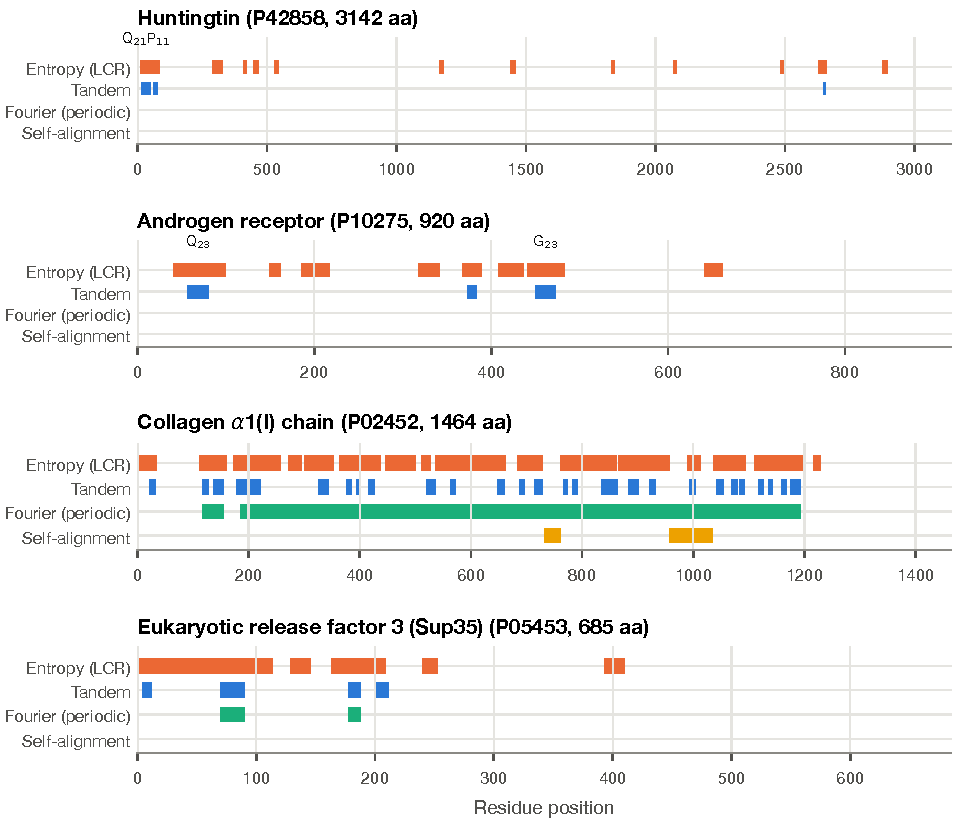
\includegraphics[height=0.86\textheight]{repeat_map.pdf}
\column{0.36\textwidth}
\small
\begin{itemize}
  \item \textbf{HTT}: \seq{Q$_{\httQLen}$} then \seq{P$_{\httPLen}$}, kept separate
  \item \textbf{AR}: \seq{Q$_{\arQLen}$} (\arQStart--\arQEnd) and \seq{G$_{\arGLen}$} (\arGStart--\arGEnd)
  \item \textbf{COL1A1}: period-3 helix, visible only to Fourier
  \item \textbf{Sup35}: \seq{\supUnit} unit; diverged copies need alignment
\end{itemize}
\end{columns}
\end{frame}

% ---------------------------------------------------------------- 12
\begin{frame}{Strengths and blind spots}
\centering
\footnotesize
\renewcommand{\arraystretch}{1.2}
\begin{tabularx}{\textwidth}{@{}l>{\raggedright\arraybackslash}X>{\raggedright\arraybackslash}X@{}}
\toprule
& \textbf{Detects well} & \textbf{Misses or misleads} \\
\midrule
Entropy & Homopolymers, compositional bias; linear time & Diverged/domain repeats; flags non-repeats \\
Self-match & Exact tandem units and copy number & Distributed repeats; variable positions; indels \\
Fourier & Periodic architecture without identical units & Period 1; non-periodic \& distributed repeats \\
Self-alignment & Diverged copies with indels; significance & Very diverged domains; LCR-dominated unless masked \\
\bottomrule
\end{tabularx}

\bigskip
\normalsize
\alert{Recommended pipeline:} entropy $\rightarrow$ self-match $\rightarrow$ Fourier $\rightarrow$ masked self-alignment
\end{frame}

% ---------------------------------------------------------------- 13
\begin{frame}{Functional implications}
\begin{columns}[T]
\column{0.48\textwidth}
\textbf{Protein folding mechanisms}\\
\small Domain repeats stack into solenoids (HEAT, ankyrin, LRR); collagen needs Gly at every third position.

\medskip
\normalsize\textbf{Evolutionary conservation patterns}\\
\small Slippage and unequal crossing-over change copy number rapidly; Sup35 repeat number tunes prion propagation.
\column{0.48\textwidth}
\textbf{Neurological disease associations}\\
\small PolyQ expansions: Huntington's disease (HTT, $\ge$\,36--40 CAG), spinal and bulbar muscular atrophy (AR), spinocerebellar ataxias.

\medskip
\normalsize\textbf{Potential therapeutic targets}\\
\small Huntingtin-lowering antisense oligonucleotides have been tested in patients; expanded proteins are targets for lowering expression or aggregation.
\end{columns}
\end{frame}

% ---------------------------------------------------------------- 14
\begin{frame}{Conclusion}
\begin{itemize}
  \item No single method finds every repeat: \alert{the repeat class determines the method}
  \item Entropy and self-match recover disease-associated polyQ tracts exactly
  \item Only Fourier analysis reveals the Gly-X-Y periodicity of collagen
  \item Self-alignment finds diverged repeats, but only after \alert{low-complexity masking}
  \item Open, tested implementation: \texttt{aarepeats} (Python), all figures reproducible
\end{itemize}
\end{frame}

% ---------------------------------------------------------------- end
{\setbeamercolor{background canvas}{bg=ink}
\begin{frame}[plain]
\centering\vfill
{\color{paper}\Huge\bfseries Thanks For your Attention}\\[1.2em]
{\color{accent!60}\large Ali Ahmadi Esfidi \quad·\quad Feb, 2025}
\vfill
\end{frame}}

\end{document}
